%----------------------------------------------------------------------------
\chapter{Firmware}
%----------------------------------------------------------------------------


Az előző fejezetekben bemutattam a robot modelljét, és vezérlésének terveit. Volt
szó az alkalmazott szenzorokról és motorokról, bemutatásra került a tápegység, és
a robot mechanikai váza.

Ebben a fejezetben a mikrokontrolleren futó program, a firmware működését fogom
bemutatni, kezdve annak specifikációjával és szükségességével. Bemutatom a
firmware létrehozásához használt build rendszert, a firmware architektúráját, és
működését. A fejezet végén kitérek a továbbfejlesztési lehetőségekre is.

\section{Specifikáció}

\subsection{Target platform}

A robot hardverének meghajtásáért felelős mikrokontroller, a robot hardveres
komponenseinek közvetlen vezérléséért felelős, a rajta futó firmware minősége a
robot működése szempontjából kritikus. Ennek a programnak a feladata a robot
hardvereinek összekapcsolása a robot szoftveres részével. Működése szoros
kapcsolatban áll a meghajtott hardver működésével és időzítése kritikus a feladat
szempontjából így igény van real-time működésű firmware kialakítására.

Az STM32F103 mikrokontroller egy 32 bites ARM Cortex-M3 magot tartalmazó
mirovezérlő. Modern kialakításának és gyártói támogatásnak köszönhetően C nyelven
programozható chip. A vezérlő 60 kB flash memóriát, és 20 kB RAM memóriát
tartalmaz, ezek a firmware számára betartandó keretek a programkód mérete és a
program szervezése és memórialábnyoma szempontjából.

\subsection{A Firmware feladatai}

Tekintsük át a firmware feladatait!

\begin{itemize}
\item{Kommunikáció a Raspberry Pi-vel}
\item{Szenzorok inicializálása és kezelése}
\item{Motorok vezérlése}
\item{Motorok sebességének mérése}
\end{itemize}

\subsection{A kommunikáció és protokol}

Az első feladat a kommunikációs csatorna defíniálása. A firmware a hardvert a
magasabb szintű logikától kapot utasítások alapján vezérli, ezért kialakításnál
master-slave jellegű kommunikációs megközelítést célszerű alkalmazni.

A kommunikáció soros porton keresztül történik. Ezen a csatornán bájtos
adatátvitel lehetséges, ezért üzenet alapú kommunikációt használtam. Az
üzenetváltás során meghatároztam parancs és legkérdezés üzeneteket, amelyeket a
Raspberry Pi küld információ kérés vagy vezérlés céljából. A kapott üzenetre a
firmware egy üzenetben választol, annak függvényében, hogy a parancsot nyugtázta
(ACK) vagy ismeretlennek találta (UNKNOWN). Ha a parancs lekérdezés volt, úgy a
mikrovezérlő válaszol a kért adattal egy üzenetben. A zárásként a mikrovezérlő
lezárja az üzenetváltást egy DONE üzenettel.

Az üzenetek egy vagy több bájtot, vagyis karaktert tartalmazhatnak, és
mindenképpen carriage-return karakterrel végződnek. Egy transzfer a fent
ismertetett üzenetváltásból áll, minden esetben egy parancsal kezdődik és egy
DONE jelzéssel (hiba esetén UNKNOWN jelzéssel) ér véget.

A kommunikációra csak ASCII karakterek használhatóak, ezzel elkerülve, hogy az
adatbájtok véletlenül egybeessenek a sor vége karakterrel, és így idő előtt
megszakítsák a kommunikációt.

\begin{figure}
  \centering
  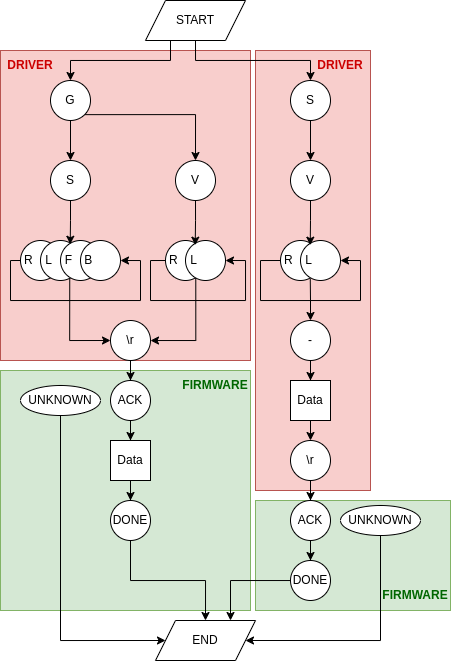
\includegraphics[width=100mm, keepaspectratio]{figures/ch3/protocol.png}
  \caption{A kommunikációs protokol}
  \label{fig:protocol}
\end{figure}

Tekintsük át a lehetséges üzeneteket. A firmware feladatainak defíniálásakor
tisztázódott, hogy kétfajta üzenet létezik, SET vagy GET, amely valamilyen
adatot mint érték kér, vagy vezérlő üzenet és a firmware valamely paraméterét
állítja. Ezeket az üzenetben rendre `s' vagy `g' karakter jelöli.

A mikrokontroller szenzorokkal távolságot mér, illetve enkóderek segítségével a
motorok sebességét. Ezáltal GET utasítás sebességre, és távolságra adható, ezeket
az üzenetben VELOCITY `v', illetve SENSOR `s' karakter jelöli. A továbbiakban
target-ként hivatkozom rájuk. SET parancs
értelemszerűen csak sebességre adható, így SET parancsot csak VELOCITY target
követhet: ``sv''.

A parancsot ezek után SENSOR target esetén maximum négy, VELOCITY target esetén
maximum két iránymeghatározó karakter követi. Ezek a FORWARD, BACKWARD, LEFT,
RIGHT irányhatározó rendre a `f', `b', `l', `r' karakterekkel. VELOCITY target
esetén csak LEFT és RIGHT irányhatározó karakter érvényes, lévén a robot két
motorral rendelkezik. 

GET parancs esetén az üzenetet carriage-return karakterrel zárhatjuk, és a
specifikált sorrendben várhatjuk a mikrovezérlő válaszát. Amennyiben SET
parancsot adtunk, úgy egy `-' karakterrel jelezzük a firmware számára hogy adat
következik. A küldendő adatot hexadecimális formában ASCII karakterekre kódolva
abban a sorrendben küldjük el, amely sorrendet az irányhatározó karaktereinkel
meghatároztunk. A megfelelő mennyiségű adat elküldése után a mikrovezérlő
nyugtázza a megkapott utasítást (ACK), majd annak végrehajtásáról DONE üzenetben
tájékoztat minket.

GET parancs esetén a firmware ugyanilyen formátumban biztosítja számunkra az
adatot. Az UNKNOWN, DONE és ACK üzenetek karaktereit rendre a `u', `n' és `k'
karakterek jelölik.

\medskip

\subsection{Szenzorok inicializálása és lekérdezése}

A firmwarenek feladata a szenzorok inicializálása. A mikrokontroller egy I2C
perifériát használ a szenzorok kezeléséhez, viszont mindegyik szenzorhoz
egyesével tartozik egy GPIO, amelyel a szenzor bootolása vezérelhető. A szenzorok
adatlapjából kiolvasható, hogy boot után a 0x52 címen érhetőek el. A bootfolyamat
késleltetésével a firmware fel tudja paraméterezni külön-külön az összes
szenzort, így azok a futás alatt saját címmel rendelkezhetnek.

Az inicializáció után a firmware aszinkron módon gyűjt adatot a szenzoroktól
amelyeket parancsra elérhetővé kell tennie a Raspberry számára. Ezzel az
architektúrával elkerülhető, hogy feladatok véletlenszerű felhalmozódása
bottlenecket képezzen a rendszerben, viszont megfelelően gyakori leolvasás esetén
megközelítőleg ugyanolyan pontos működést kapunk.

\subsection{Motorok sebességének mérése}

A mikrovezérlő dedikált timer perifériákat tartalmaz amelyek külön funkcióval
rendelkeznek az inkrementális enkóderek jeleinek feldolgozásához. A timerek
megfelelő inicializációja után a firmware feladata kiolvasni a timerek cnt
regiszterének értékét, majd ezekből az értékekből a robot sebességét valamilyen
algoritmus segítségével kiszámolni.

A sebesség algoritmusa függ a felhasznált alkatrészek fizikai paraméterétől, mint
a kerék átmérője, a motorokon használt áttétel, az enkódertárcsák beosztása,
valamint, ha a differenciális elrendezésből egy sebességértéket szeretnénk
defíniálni, a kerekek egymástól vett távolsága.

A sebességmérés pontossága függ az enkóder felbontásától, a kerék aktuális
szögsebességétől, valamint a lekérdezés időbeli pontosságától is.

A sebesség mértékegysége előre meghatározandó paraméter amit a firmware számára
specifikálni kell. Ezt a mértékegységet a robot léptékeihez és a feladatához
mérten mm/s egységben állapítottam meg.

\subsection{Motorvezérlés}

A motorok sebességének beállítása szintén a firmware feladata. A sebesség
beállítás komplex feladat is lehet, amennyiben nagy pontosságra törekszünk.

A motorok sebességszabályozásért felelős algoritmus állhat egy egyszerű PWM
állításból de egy komplex PID szabályzóból és szabályzókörből is. Az algoritmus
komplexitásának felső korlátja, hogy egy iteráció futásideje bele kell, hogy
férjen a szabályzó task periódusidejébe, amit a floating point unit hiánya
nagyban meg tud nehezíteni bizonyos sebesség felett.

A firmware specifikációja során nem határoztam meg pontos követelményeket, és a
végső kialakításban nem szerepel PID szabályzás, de a kódbázisban implementálva
van egy szabályzó, ami alkalmas lehet további fejlesztésre.

\medskip

A motor vezérlésénél fontos kérdés, hogy mi történjen ha elveszik a kapcsolat a
magasabb szintű vezérléssel. Robotikai alkalmazásokban általános megoldás, hogy
ilyen esetben a robot megáll, hiszen a funkcionalitás jelentős része kiesett, így
a robot akár károkat is okozhat. A folyamatos kapcsolat igényét a firmware
fejlesztése során szem előtt tartottam.

\begin{figure}
  \centering 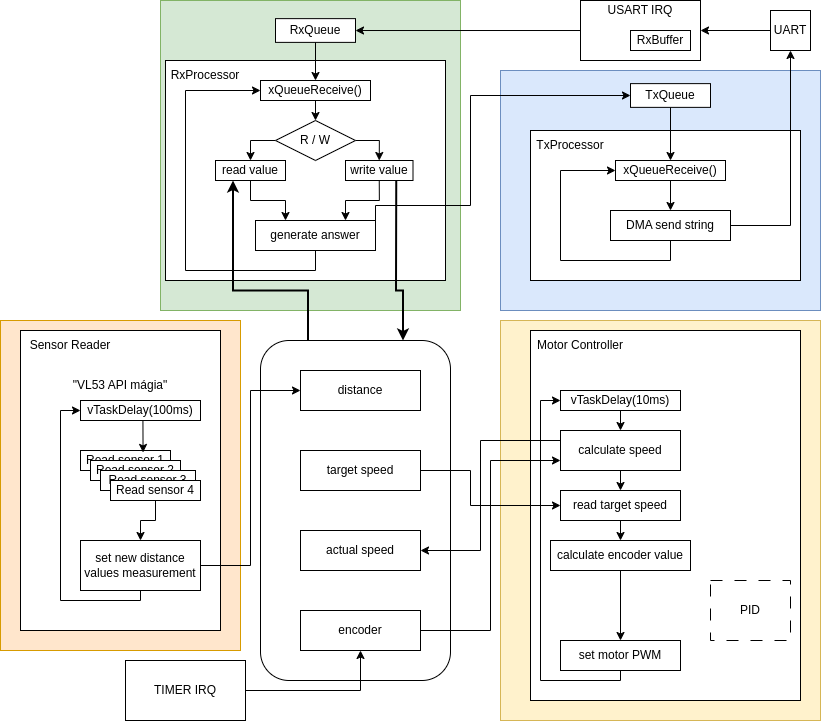
\includegraphics[width=150mm,
    keepaspectratio]{figures/ch3/firmware-architecture.png}
  \caption{A firmware blokkdiaggramja}
  \label{fig:firmware_arch}
\end{figure}

\section{Build}

A szoftverfejlesztés egy fontos eleme, hogy az adott build artifact könnyen
reprodukálható legyen. Az összetett fejlesztőkörnyezetek integrált toolchainjei
és komponensei ezeket a funkciókat általában megnehezítik, és megkötik a
fejlesztő kezét a felhasznáható eszközök terén.

A firmware fejlesztése alatt különleges figyelmet fordítottam rá, hogy munkám
széles körben elérhető eszközöket igényeljen csak a fordításhoz, és minél
modulárisabb, könnyebben cserélhető eszköztárra és projektkomponensekre bontottam
a feladatot.

A fordításhoz a GNU toolchain ARM mikrokontrollerek számára készült verzióját, az
\verb|arm-none-eabi-gcc|-t használtam. A többlépcsős build folyamat
végrehajtásához shellscriptekből és Makefileokból álló rendszert építettem, amely
a forráskódot viselkedés szerint modulokba engedi csomagolni, így többfajta
kialakítású projekt is könnyedén integrálható a buildbe. A nyelvi szerver
támogatáshoz \verb|clangd|-t használtam amihez a szükséges
\verb|compile_commands.json| file-t a \verb|bear| nevű, szintén open source
szoftverrel generáltam.

A projekt ezen felépítése lehetővé teszi hogy tetszőleges editorral (vim, emacs,
vscode) vagy fejlesztői környezettel megnyitható és szerkeszthető legyen.

A project teljesen verziókövetve van amihez git-et használtam. A repository
szabad licensz mellett elérhető a github linken\cite{RpirobotGitrepo}. 

\subsection{A project architektúrája}

A repository root könyvtárában két fontos mappát találunk, a \verb|utils| és
\verb|modules| mappákat. A \verb|utils| mappa tartalmazza a projekthez használt
általános scriptek legnagyobb részét. Ebben a mappában található scriptek a
következők:

\begin{itemize}
\item{build.sh:~A build folyamatot elindító script.}
\item{clean.sh:~A build artifactokat törlő script.}
\item{flash.sh~Az elkészült binárist ST-Linken keresztül a mikrokontrollerre
  másoló script.}
\item{openocd-start:~Az openocd service indító scriptje, amely on-chip
  debugoláshoz használandó.}
\item{openocd-start-bg:~Az openocd service indító scriptje, amely on-chip
  debugoláshoz használandó. A folyamatot háttérfolyamatként indítja.}
\item{gdb.sh:~Az arm gdb programot megfelelő indítási kapcsolókkal indító script,
  igényli az openocd futását.}
\item{gdb-ide.sh:~Az arm gdb programot megfelelő indítási kapcsolókkal a
  fejlesztőkörnyezetből indító script, igényli az openocd futását.}
\item{stm32f1x.cfg:~Az openocd által igényelt konfigurációs file a target
  mikrovezérlőhöz.}
\end{itemize}

A build egyszerűen végrehajtható a \verb|build.sh| script futatásával. A buildhez
tartozó konfigurációt a \verb|settings.sh| file tartalmazza, ami a repository
root könyvtárában található. A scriptben néhány hasznos beállítás amit
konfigurálni lehet:

\begin{itemize}
\item{A projekt neve}
\item{A fordító és linker binárisok}
\item{A kimenetet tartalmazó könyvtár}
\item{A fordításhoz és linkeléshez használt flagek}
\item{Az optimalizáció szintje}
\item{A lefordítandó modulok listája}
\end{itemize}

A projekt root könyvtárában található modules mappa további mappákat tartalmaz,
amelyek a projektben használt modulok.

A moduláris kialakításnak hála, egy új szoftverkomponens vagy library lefordítása
sokkal könnyebb és nem borítja meg a projekt addigi architektúráját. Egy modul a
modules mappán belül található olyan könyvtár amely tartalmaz \verb|module.sh|
scriptet.  A \verb|module.sh| script minden modulhoz meghatározza a fordítás
lépéseit, ami a leggyakrabban egy make parancs. A modul saját mappájában belül
dolgozik, és kimenetét egy obj nevű mappában gyűjti össze. A modul lefordulása
után ezek a kimenetek a modul nevének prefixálásával bemásolásra kerülnek a
projekt \verb|build| mappáján belül található \verb|obj| mappába. Ezzel a megoldással
elkerülhetjük, hogy két modul által ugyanazon a néven hívott object file
felülírja egymást.

A modulok jellemzően tartalmaznak egy \verb|Makefile|-t is, ami a pontos build
instrukciókat és a függőségeket is tartalmazza.

A modulok lefordítása és kimeneteik globális build mappába történő másolását
követően a build script meghívja a \verb|Make|-et a project root könyvtárából, ami a
linkelést elvégzi. Az így kapott kimenet egy ``.elf'' file, amely mellé
automatikusan generálódik egy ``.bin'' kiterjesztésű file, ami alkalmas a
mikrokontrollerre történő másolásra.

\medskip

A build folyamat végeztével az ST-Linket csatlakoztatva a fejlesztői
számítógéphez, a \verb|utils/flash.sh| scriptet futtatva a program letölthető a
mikrovezérlőre. 

\section{Felhasznált libraryk és keretrendszerek}

A firmware fejlesztéséhez több könyvtárat és eszközt használtam a projekt
áttekinthetősége, és a fejlesztés sebessége végett. A következőkben röviden
bemutatom a projektben használt librarykat és keretrendszereket. Röviden
bemutatom lényegi működésüket, indoklom szükségességüket a projekt szempontjából,
és kitérek előnyeikre és esetleges nehézségeikre is.

\subsection{FreeRTOS}

A firmware-ek felhasználási területükből kifolyólag gyakran real time
működésűek. Egy real time működésű program garanciát vállal, hogy meghatározott
időn belül biztosan választ ad. A real time működés elérését gyakran
nehezíti, hogy egy mikrovezérlő programja több feladatkört lát el egyidőben. Az
ilyen típusú multitasking környezetek megsegítésére real time
operációsrendszereket alkalmazunk.

Egy real time operációsrendszer nem garantálja a szoftver real time működését,
viszont lehetővé teszi, hogy real time működésű szoftvert fejlesszünk. Az
operációsrendszer eközben eszközkészletet biztosít a fejlesztő számára
a multitasking megkönnyítésére és a versenyhelyzetek, és IPC\footnote{IPC:~Inter
Process Communication} igények kezelésére. A firmware feladatainak
számából adódóan szükségesnek láttam egy operációsrendszer használatát.

Mikrokontrolleres alkalmazások tekintetében a legelterjedtebb beágyazott
operációsrendszer a FreeRTOS, amely egy ingyenes, nyílt forráskódú RTOS, 32 bites
mikrokontrollerekre lett tervezve.

A FreeRTOS operációsrendszer számos hasznos eszközt biztosít:

\begin{itemize}
\item{Konfigurálható kernel, többfajta ütemező algoritmussal.}
\item{Mutexek és szemaforok, szinkronizáció, és versenyhelyzetek kezelése
  céljából.}
\item{Opcionális dinamikus memóriakezelés, malloc, és free implementációkkal.}
\item{Taskok, Task prioritások, Taskkezelő mechanizmusok, függvények.}
\item{Message Queue-k, Notificationok, IPC megoldások.}
\end{itemize}

A firmware első modulja (a main modult leszámítva) a FreeRTOS modul. Ez a projekt
forráskód szinten elérhető, és rendkívül jól dokumentált. A FreeRTOS monolitikus
kialakítású, az operációs rendszer egybe fordul a projektel. A main függvényben a
``vStartScheduler()'' függvényhívással indíthatjuk el az ütemezőt. Amely ezután
ütemezi az előzőleg létrehozott taskokat.

Az operációsrendszer funkcióihoz API hívásokon keresztül férünk hozzá, ezek vagy
függvények vagy makrók formájában állnak rendelkezésre. A FreeRTOS beállításait
egy FreeRTOSConfig.h nevű headerben találjuk, ehhez a filehoz referencia
implementációt a FreeRTOS honlapján a dokumentációban találhatunk. Fejlesztés
előtt érdemes a rendszerrel megismerkedni, és a használni kívánt rendszerhívások
dokumentációját átolvasni, erre a FreeRTOS honlapján az API
reference\cite{FreertosApiReference} szolgál.

\subsection{CMSIS}

Az ARM minden gyártótól aki ARM licenszelt architektúrát implementál megköveteli,
hogy termékük mellé készítsenek CMSIS támogatást. A CMSIS, azaz Cortex
Microcontroller Software Interface Standard, egy szabvány amely az eszközhöz
regiszterdefiníciókat és alapszintű működéshez tartozó függvényeket
biztosít. Segítségével elkerülhető, hogy a fejlesztést megelőzően minden
regiszterhez saját definíciót kelljen készítenie a fejlesztőnek, vagy a driver
kódban mágikus konstansokat használjon regisztereléréshez.

\medskip

A CMSIS a hardverhez legközelebbi szint, ahol olvasható kódot lehet C nyelven
írni. Érdemes megemlíteni, hogy csak CMSIS felhasználásával és egyéb absztrakciós
rétegek nélkülözésével rendkívül optimális kód írható. Erre a szintű
optimalizálásra azonban csak nagyon ritkán van igény, mert az adott feladathoz
használt mikrovezérlő rendszerint jelentős erőforrástartalékkal rendelkezik, így
a fejlesztést könnyítendő nincs szükség mikrooptimalizálásra. A CMSIS egyik nagy ereje,
hogy az absztrakciós library-k számára biztosít platformot. A másik fontos
alkalmazása, hogy a kód adott szegmenseiben lokálisan CMSIS kód alkalmazásával
biztosítja a mikrooptimalizálás lehetőségét a fejlesztő számára.

\medskip

A projekt keretein belül limitált mennyiségben használtam direkt CMSIS kódot,
lévén nem merült fel komoly igény ilyen mértékű mikrooptimalizálásra. Az aktuális
firmware fejlesztését megelőzően azonban volt kísérletem CMSIS alapú kód
fejlesztésére, amelyet a fejlesztés sebessége miatt nem tartottam ideálisnak,
ezért azt a projektet elvetettem, és új alapokra helyeztem a robot firmware
kódját.

\subsection{HAL}

Az STMicroelectronics biztosít két absztrakciós réteget a mikrovezérlőihez, ezek
az LL driver, valamint a HAL\footnote{HAL:~Hardware Abstraction Layer} driver. A HAL
driver egy magas szintű hardver absztrakciós könyvtár, amely minden STM32
perifériához tartalmaz driver réteget. A HAL kód könnyebben olvasható mint egy
CMSIS ellenben teljesítményében lassabb, és számottevően nagyobb méretű kódra
fordul.

A projekt fejlesztése során a HAL drivereket és saját kiegészítő kódot használtam
a mikrovezérlő hardvereivel történő interakcióban, ennek három fő indoka volt.

\begin{itemize}
\item{A HAL Driverek jól dokumentáltak, sok segédanyag érhető el velük
  kapcsolatban}
\item{Az STMicroelectronics CubeMX eszköze a HAL kód generálását támogatja.}
\item{A HAL Driverek felahsználásával lényegesen gyorsabban tudtam működő kódot
  létrehozni.}
\end{itemize}

Az STMicroelectronics biztosít egy fejlesztés segítő eszközt, az STMCubeMX
kódgeneráló és lábkiosztás menedzser programot. Ez a program integrálva elérhető
a CubeIDE fejlesztői környezetben, illetve standalone verziója is beszerezhető a
gyártó honlapjáról. A HAL driverek mellett szóló erős érv, hogy a projekt
inicializációja során a CubeMX által generált inicializáló kód nagyban
megkönnyítette a projekt bootstrapelését.

\medskip

A HAL driverek felhasználásának akadnak azonban hátrányai is. Ipari
alkalmazásában bizonyos feladatok megkövetelik, a HAL Driverek adott funkcióinak
helyettesítését. Erre a fejlesztés során közvetlen példát találtam.  USART stream
olvasása során a robot esetében számolni kellett azzal, hogy billentyűzetről
történő olvasással ellentétben a stream karakterei között nem lesz üres idő, és
egy karakter megérkezése után a következő karakter fogadása már folyamatban
van. Egy ilyen stream fogadását DMA vagy interrupt rutinok segítségével lehet
megvalósítani, ahol viszont az interrupt rutinnak megfelelően rövid idő alatt
kell lefutnia.

Pusztán HAL driverek felhasználásával ez nem lehetséges, mert az interruptos
olvasás újboli bekapcsolása a driverben reseteli az USART perifériát, amely így a
következő karaktert frame errorral fogja olvasni.

\subsection{VL53L1 API}

A VL53L1 szenzor egy teljes mikrovezérlőt magában foglaló távolságmérő eszköz,
meghajtása jelentősen eltér az I2C interfésszel rendelkező szenzorok döntő
többségétől. A projektbe történő integrálás során ez többször jelentett nagyobb
megakadást is.

\medskip

A VL53L1 szenzor, rengeteg belső funkcióval és konfigurációs lehetőséggel
rendelkezik, vezérlése komplex feladat. Az STMicroelectronics erre a problémára
válaszul kiadott egy forráskód szinten elérhető driver csomagot, amely
lefordítható tetszőleges architektúrára, és a szenzor vezérlését végzi.

A projekt során a szenzorok illesztésének feladata lényegétben ennek a drivernek
a beágyazása és lefordítása volt.  A driver több mint 30 forrásfile-ból áll, a
csomagban található dokumentáció valamint rövid readme, amely a driver
felhasználását hivatott bemutatni. A csomag implementál minden fontos vezérlő
logikát amely a szenzor vezérléséhez szükséges, ezekhez pedig publikus API
tartozik, amely függvények dokumentálva vannak a driverhez mellékelt API
dokumentációban. A driverben az I2C interfész kezelésére szolgáló függvények
nincsenek implementálva, ezek csak szimbólum szinten jelennek meg. Az integrálás
legfontosabb része ezeknek a függvényeknek az implementálása, amely a driver
számára lehetővé teszi az I2C interfész használatát.

Ez a feladat jelentős nehézségeket okozott, mert nem találtam pontos
dokumentációt az implementálandó függvényekről, azok helyéről, valamint a driver
beüzemeléséről, pusztán a teljes driver használatáról.

További nehézséget jelentett, hogy a driver több verzióban is megtalálható, és
több szenzorverzióhoz készült kiadás is elérhető, a driver csomagok között pedig
tévesen időnként Microsoft Windows operációsrendszerhez szánt teszt- és
kliensprogram is előfordult.

\medskip

Alapos kutatómunkát követően végül egy STMicroelectronics fórumbejegyzésben
találtam egy verziót, amely az ULD, azaz UltraLite Driver csomag nevet
viselte. Ennek a driver csomagnak hatalmas előnye, hogy csak a legszükségesebb
forráskódokat tartalmazza, és egyértelműen defíniálva van, hogy melyik függvények
implementálását igényli.

Ez a driver verzió azért jött létre, hogy a szenzorral ismerkedő fejlesztők vagy
fejlesztőcsapatok egy könnyebben áttekinthető projekt kereteiben használhassák az
eszközt. Ennek a kiadásnak további hatalmas előnye volt a projekt szempontjából,
hogy egy nagyságrendel kisebb a lefordított kód mérete, amely így a mikrovezérlő
flash memóriájában könnyedén elfér, a firmware egyéb részei mellett.

Az UltraLite Driver lefordításában és implementációjában nagy segítségemre volt
az ULD csomagban mellékelt példa projekt. A példaprojekt kódjából kiindulva
implementáltam az I2C periféria illesztését, és sikeresen teszteltem a szenzort.

\section{A firmware architektúra}

Az előző szegmensben bemutattam a felhasznált rétegeket, drivereket, és
könyvárakat. Ebben a részben bemutatom a firmware taskfelosztását, azok
architektúráját. Bemutatom a taskok kommunikációját, valamint a robot belső
memóriamodelljét, ami a robot paramétereinek firmware-en belüli modellje. 

\subsection{A robot belső állapota}

A firmware egy singleton adatstruktúrában tárolja azokat a paramétereket amik a
robot aktuális állapotát jellemzik. A robot ilyenmódon történő modellezése egy
helyen összesíti az összes paramétert így kiegészítés során elég ezt az egyetlen
struktúrát bővíteni.

A robot paramétereinek alstruktúrákba rendeződésével, modulok szerint
tagváltozókba csoportosítható minden fontos paraméter. A kód ezért olvashatóbb és
könnyen követhető, valamint lehetőséget ad a hosszú és nem beszédes változónevek
elkerülésére. Az alstruktúrák tartalmazzák a kérdéses adatokat valamilyen
formában, valamint többségük tartalmaz mutexet, amelyet a versenyhelyzetek
elkerülésére használ a firmware.

A struktúra négy fő alstruktúrából áll:
\begin{itemize}
\item{\verb|distance|:~A szenzorok által mért adat, négy darab előjel nélküli 16
  bites egész, valamint egy mutex.}
\item{\verb|encoder|:~Az enkóderpár jelenlegi, és előző iteráció beli értékei
  előjeles 16 bites egész formában.}
\item{\verb|actual_speed|:~A robot mért sebessége ami az enkóder értékekből
  számolódik, egy pár előjeles 16 bites egész, és egy mutex.}
\item{\verb|target_speed|:~A robot célsebessége, ami egy pár előjeles 16 bites
  egész, valamint egy mutex, és egy timeout 16bites előjel nélküli egész.}
\end{itemize}

A firmware elkülöníti a mért és kívánt sebességeket. A struktúra tagjai
közül három érhető el írásra és-vagy olvasásra, a firmware számára specifikált
utasítások szerint.

\medskip

A fent bemutatott struktúrán négy task, és egy interrupt rutin végez író- vagy
olvasó műveleteket. Rendszerint egy feladat a működését befolyásoló paramétereket
a struktúrából veszi, kimenetét a struktúrába írja vissza. A kövekezőkben
bemutatom a taskokat amelyek a robot funkcionalitását adják.

\subsection{Rx Task}

A firmware az USART felől érkező utasításokat egy külön taskban dolgozza fel. Az
üzenetek fogadásához azonban egy megszakításkezelő függvényt is felhasználok.

Az USART streamen érkező utasítások karakterenként érkeznek meg a vezérlőbe,
fogadásukat interrupt rutin végzi. Egy üzenet az első karakterétől (azaz az
utolsó stop bit után számíott első start bittől) számítva a carriage-return
karakter érkezéséíg tart. Az interrupt rutin feladata, hogy minden megérkezett
karaktert egy ideiglenes bufferben tárol, majd az első ``\textbackslash{}r'' karakter
megérkezését követően az üzenetet a parancsokat feldolgozó task számára egy
message queue-ba rakja. 

A periféria 115200 baud szimbólumsebességre lett konfigurálva, ez az interrupt
rutin számára felső korlátot jelent a futásidőre nézve, hiszen az interrupt
rutinnak a következő karakter megérkezése előtt be kell fejeznie futását. Az
olvasás egy gyors művelet, ellenben a message queueban való műveletvégzés egy
rendszerhívás ami az interrupt rutin kontextusában hosszú időt vesz igénybe.

A rutin futását nehéz utasítások számából kiszámítani ezért mérést végeztem. Az
interrupt handler első sorában egy GPIO lábat 1-es állapotba állítottam,
visszatérés előtt közvetlenül pedig reseteltem, így oszcilloszkóppal az impulzus
hossszából következtettem a rutin futásidejére.

\begin{figure}
  \centering 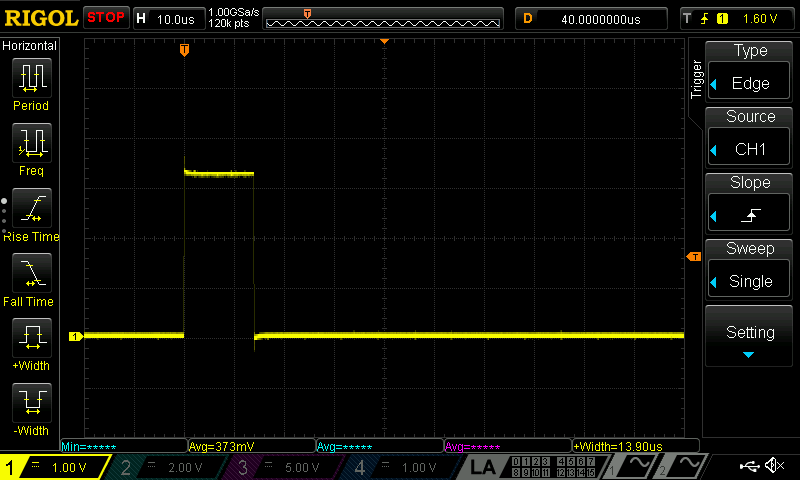
\includegraphics[width=150mm,
    keepaspectratio]{figures/ch3/osc_single_char_debug.png}
  \caption{Egyetlen karakter feldolgozásához szükséges idő debug módban}
  \label{fig:char_debug}
\end{figure}
\begin{figure}
  \centering 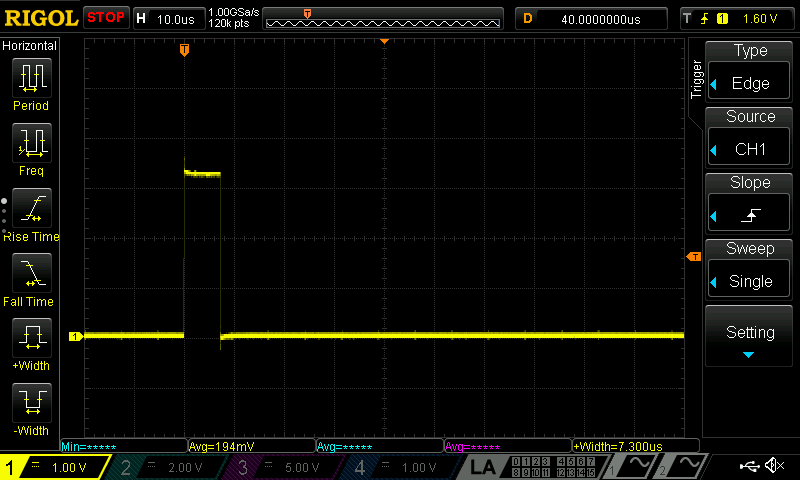
\includegraphics[width=150mm,
    keepaspectratio]{figures/ch3/osc_single_char_release.png}
  \caption{Egyetlen karakter feldolgozásához szükséges idő release módban}
  \label{fig:char_release}
\end{figure}
\begin{figure}
  \centering 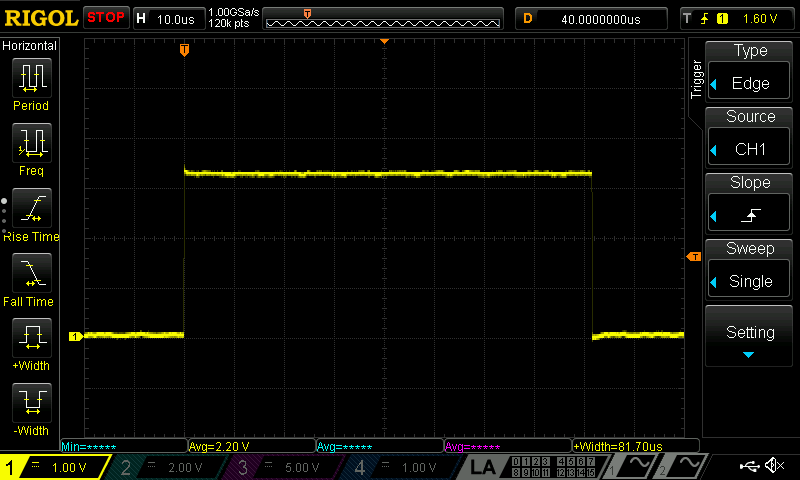
\includegraphics[width=150mm,
    keepaspectratio]{figures/ch3/osc_complete_message_debug.png}
  \caption{A kész üzenet fogadásának ideje az interrupt rutinban debug módban}
  \label{fig:msg_debug}
\end{figure}
\begin{figure}
  \centering 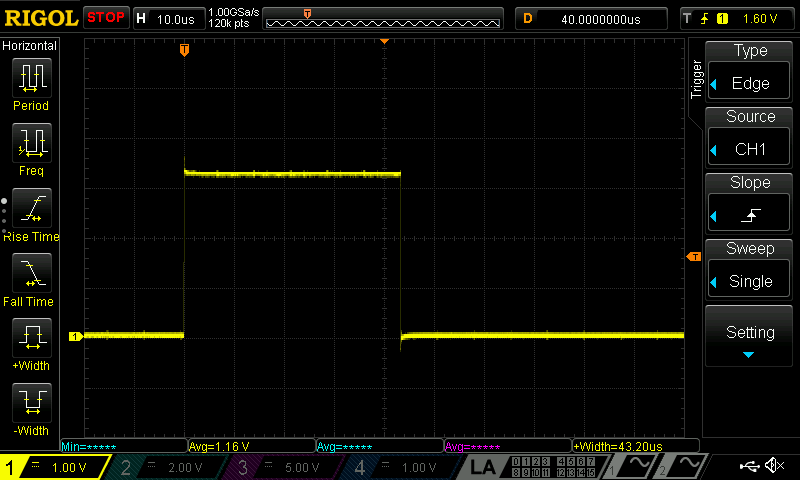
\includegraphics[width=150mm,
    keepaspectratio]{figures/ch3/osc_complete_message_release.png}
  \caption{A kész üzenet fogadásának ideje az interrupt rutinban release módban}
  \label{fig:msg_release}
\end{figure}

Az érkező karakterstream feldolgozásához szükséges feltétel, hogy a karaktereket
nagyobb sebességgel tudjuk fogadni, mint ahogyan azok megérkeznek. A szükséges
idő limitet a következő módon határoztam meg:

\medskip

Az USART konfiguráció 8N1 kialakítású, 115200 baud következésképpen az időkeret:

\begin{eqnarray*}
N_{karakter} = 10 \\
baudrate = 115200 \frac{1}{s} \\
T_{karakter} = N_{karakter} * \frac{1}{baudrate} s \approx 8.680555 * 10^{-5} s \\
T_{karakter} > 8.6 * 10^{-5} \\
\end{eqnarray*}

A fenti módszer segítségével meghatározható, a karakter-stream olvasásához
használt intterupt rutin futási idejére egy felső korlát, ezt $8.6 * 10^{-5}s$
-ban határoztam meg. A méréshez a kódot release és debug módban is lefordítottam,
az időkorlátoknak mindkét kód megfelelt. Az optimalizáció hatása látványos,
a~\ref{fig:char_debug},~\ref{fig:char_release},~\ref{fig:msg_debug},~\ref{fig:msg_release}
ábrákon jól megfigyelhető. Az interrupt rutin debug módban fordítva is 82 us
alatt fut le az üzenet endline karakterének fogadása esetében. Ez worst case
eset, amely a megállapított 86 us időnél kisebb. A kód release módban történő
futása esetén a tartalék sokkal nagyobb. 

\medskip
\textsl{
Érdekesség: A kód gyorsabb végrehajtása érdekében kísérletet tettem a függvény
flash memória helyett RAM-ból történő végrehajtására. Ennek a kísérletnek az
eredménye képpen a függvénynek az flashből történő végrehajtáshoz viszonyítva
több volt a futásideje. Ennek a jelenségnek az oka a végrehajtó architektúrájában
keresendő, a RAM ugyanis a harward architektúrának megfelelően nem a
kód végrehajtásra lett tervezve, így az utasítások felolvasása lassabb, még ha a
RAM sebessége elméletben a flash sebességénél nagyobb. Komplexebb
mikrovezérlőkben, amelyek nagyobb órajelfrekvencián működnek, ilyen esetekre egy
kis méretű utasítás-úti RAM modul is megtalálható, ahova a nagy sebességben
végrehajtandó kód betöltésre kerül.
}

\medskip

Fontos kiemelni, hogy a karakter stream időkorlátjának teljesítése nem elégséges
feltétele a helyes futásnak, a rendszernek ugyanis időre van szüksége a parancsok
értelmezéséhez és végrehajtásához is. Ennek érdekében egy message queue-t
alkalmaztam, amely egy FreeRTOS funkció. A message queue eltárol maximum 5
stringet, amelyeket a parancsfeldolgozó task kiolvas, és végrehajt. A queue
feltöltését az interrupt handler rutin végzi minden fogadott `\textbackslash{}r'
karakternél. A queue hatására rövid ideig tartó message burst-öt a firmware képes
lekezelni, és az üzenetekre érkezési sorrendben reagálni. 

\medskip

A parancsokat értelmező task az inicializációs fázist követően várakozik a
message queue-ba érkzező üzenetekre, amennyiben üzenet érkezik, úgy azt
végrehajtja. A parancsok a specifikációnak megfelelően értelmeződnek. Külön
függvényben történik a beérkező parancs értelmezése és bírálása, hogy
értelmezhető vagy ismeretlen utasítás. Értelmes utasítás hatására egy parancs
struktúra generálódik. A parancs állapotáról a task visszajelzést küld, ennek
végrehajhatósága esetén a generált parancs struktúrát egy végrehajtó függvény
kezeli, amely az állapotot módosító függvények meghívását végzi. 

\subsection{Tx Task}

A fogadást végző feladattól külön választva, egy sokkal egyszerűbb kialakítású
task kezeli az üzenetek küldését. Programszervezés szempontjából logikusabbnak
láttam, ha a küldés és fogadás külön taskokon keresztül történik.

A task felépítésében hasonlít fogadást végző társára, az elküldendő üzenetek egy
szeparált message queue-ba érkeznek, amelyből a task érkezés sorrendjében kiveszi
majd elküldi az üzeneteket.

Az üzenetek küldését a processzoridővel való takarékoskodás jegyében DMA
felhasználásával végeztem, így a task futásideje alacsonyan tartható. 

\medskip

A taskok inicializációjának sorrendjében megfigyelhető függőség, például az
RxTask nem válaszolhat, amig a küldést végző task nem fejezte be inicializációs
lépéseit. Ennek a befolyásolására a taskok létrehozásának sorrendje alkalmas
megoldás. Ez a megközelítés azonban olyan megoldáshoz vezet, ami a forráskódból
nehezen olvasható logikát implikál, a firmware esetleges átstruktúrálására a
rendszer érzékennyé válik.

Alternatív megoldásként a taskok inicializációs lépéseit kiegészítettem
szemaforok felhasználásával, amelyek segítségével a függő taskok blokkolnak,
ameddig függőségeik nem teljesülnek. Ennek a kialakításnak kis mértékben nagyobb
memóriaigénye van, lévén a taskokat szinkronizáló szemaforoknak szükséges
memóriaterület, de robosztusabb megoldás ami látványosabb is a kód olvasása
közben.

\subsection{Motor Task}

A motor vezérléséért felelős tasknak két fő feladatot kell ellátnia. A motor
sebességének vezérléséhez a PWM kitöltési tényezőt ki kell számítania, illetve a
motorok sebességét is ki kell kalkulálnia.

\subsubsection{Sebességmérés}

A sebesség pontos méréséhez egy timer periféria megszakítását használtam, lévén
az enkóder timerek perifériáinak olvasását minél pontosabban, azonos időközönként
kell olvasni. A megszakításkezelő rutin egy egyszerű feladatot végez, minden
meghívás alkalmával a robot paramétereit tároló globális struktúra enkóder
mezőjét frissíti. Mindkét motorhoz tartozó enkóder timer CNT  regiszterét
kiolvassa, majd az eltárolt előző értéknek beállítja az eltárolt jelenlegi
értéket, ezt követően a számlálóból kiolvasott értékkel frissíti a jelenlegi
számlálóértéket. A megszakítás kezelő értelemszerűen mindkét motor sebességét a
fenti módon frissíti. A rutin semmilyen többletfeladatot nem végez, mert az
időkritikus pont az új mérési eredmény pontos időben történő megszerzése, a
számítások elvégzésére a motorvezérlő task tökéletesen alkalmas.

\medskip

A motorok vezérlésének első lépése a sebesség meghatározása. Ezt az imént
bemutatott módon, az interrupt által kiolvasott enkóder értékekből végzi a
firmware. Az interrupt rutin csak kiolvassa a sebességet, azonban a task szintén
a rutin által írt memóriaterületet olvassa ami versenyhelyzetet eredményez. Arra
az időre, amig a task kiolvassa a robot paraméterei közül az enkóder értékeit,
kritikus szakaszt határoztam meg. Ennek a megközelítésnek nagy előnye, hogy nem
igényel mutex létrehozást, ami az időzítést tovább nehezítené, ellenben a
kritikus szakasz olyan rövid, hogy nincs lényegi ráhatással a rendszer többi
komponensének idejére. A kritikus szakaszban töltött idő alatt beérkező
megszakítások a szakaszból történő kilépéssel érvényre jutnak, így nem 
maradhat ki megszakítás sem.

A sebesség meghatározását ezek után egy egyszerű matematikai képlet segítségéve a
task már könnyedén elvégzi, a kiolvasott enkóderértékek, a kerék és motor fizikai
paraméterei és a megszakítás periódusideje alapján:

\begin{eqnarray*}
CNT = \text{az enkóder értéke} \\
N_{inkremens} = 14 \\
D_{kerék} = 21 mm \\
C_{kerék} = D * \pi \\
G_{áttétel} = \frac{1}{100} \\
t = 10 ms \\
s = \frac{C_{kerék} * CNT}{N_{inkremens} * G_{áttétel}} \\
v = \frac{s}{t} \\
\end{eqnarray*}

Tehát a kerék kerülete az átmérőből adódik, az enkóder egy teljes körülfordulás
alatt 14 lépést végez, a motor áttétele pedig egy tényleges körülfordulást 100
motortengely fordulással ér el. A CNT értékével skálázva megkapjuk a kerék által
megtett utat, amit a mintavétel periódusidejével leosztva megkapjuk a
sebességet.

A sebesség mértékegységének a mm/s mértéket választottam, amely a robot
feladatához  és méretéhez viszonyítva alkalmas méretarányban reprezentálja a
motorok sebességét.

A motor, áttétel, vagy kerék cseréje esetén a paraméterek újbóli megadása
szükséges, ezt a jelenlegi firmware verzióban egy header file-ban lehet
konfigurálni. 

\subsubsection{Sebességszabályozás}

A motor sebességének szabályozására az eredeti tervekben PI, vagy PID szabályzó
szerepelt. A firmware végleges megvalósításában a szabályzás megvalósítására már
nem maradt idő, ellenben a kód szerkezetének kialakításában figyeltem rá, hogy a
szabályzás könnyen integrálható legyen.

A projektnek része egy szabályzó algoritmus, amelyet külső könyvtár
részeként\todo{hivatkozás} integráltam a projektbe, a kód viszont nem került
végrehajtásra.

\todo{leírjam a szabályzás menetét, szabályzóhangolást?}
\todo{szabályozáshoz irodalomhivatkozás, jegyzet?}

A motor sebességszabályozása jelenleg a beállított sebességérték mint PWM jelet
vezérlő jellemző kerül direkt beírásra a timer ARR\footnote{ARR:~AutoReload Register}
regiszterébe. Ez a kialakítás a vezérlő logika számára lehetővé teszi a pontos
PWM beállítást, ellenben a hardverhez túlságosan közeli hozzáférést biztosít, ami
nem elegáns megoldás, lévén a firmware feladatai között szerepel a hardver
absztrahálása.

\subsection{Sensor Task}

Végül de nem utolsó sorban a firmware tartalmaz egy szenzor vezérlő taskot. Ennek
a tasknak a feladata a VL53L1 szenzorok inicializálása, egyedi címek kiosztása,
valamint a szenzorok periodikus olvasása, az UltraLite driveren keresztül.

\medskip

A task kezdeti lépésben négy címet hoz létre, amivel a szenzorokat
inicializálja. Az inicializáció során a szenzorokat a hozzájuk rendelt GPIO
lábakon keresztül egyesével, egymás után bootolja be, majd egyedi címmel látja el
őket. A már bebootolt szenzorok csak a nekik kiosztott egyedi I2C címekre fognak
válaszolni, így a soron következő eszközt alapértelmezett gyári címén megszólítva
az inicializáció elvégezhető. A sensorok helyes működéséről és állapotukról
visszajelzést adnak, amit polling jellegű megoldással, driver támogatással
vizsgál a task.

Az összes szenzor bebootolását követően a task fő ciklusában egyesével
végigolvassa a szenzorokat, amelyek, amennyiben van elérhető mérési adat, azt
visszaküldik a vezérlő fele. A szenzorolvasó task ezt követően a robot
paramétereinek struktúrájába, a megfelelő alstruktúrába beírja az értékeket. A
struktúra mutexel védett, lévén a szenzorolvasó taskal párhuzamosan a
parancsvégrehajtásért felelős task olvashatja a mért távolságértékeket. 

\section{Értékelés, Fejlesztési lehetőségek}

A firmware fejlesztése összetett feladat volt, a fejlesztés során sok új
tapasztalatra tettem szert.

\medskip

Az elkészült verzió komponensei jó összhangban működnek egymással, az időzítési
feladatokat is megfelelően sikerült kivitelezni. A felhasznált hardver elégséges
volt a feladathoz, bár adott alkalmakkor a feladatot könnyítette volna egy
nagyobb teljesítményű mikrovezérlő alkalmazása.

A projekt során átható és mély ismeretekre tettem szert a fordítás, és a build
folyamatok tekintetében, az elkészült projektstruktúrát egyéb projektek
esetében is hasznosnak ítélem.  

A projekt moduláris kialakítása nagy segítség volt a fejlesztés alatt, a rendszer
átláltható, és karbantartható maradt, a javítások és kiegészítések rendszerint
könnyen megvalósíthatóak voltak.

\medskip

A projekt ezek ellenére számos hiányosságot, és fejlesztési lehetőséget is
tartalmaz. 

A robot nagy hiányossága, hogy a motorok szabályozása nincs implementálva. A
szabályzás implementálásához a motorokon rendszeridentifikációt kell végezni,
majd az így kapott rendszerhez PID szabályzót hangolni. A paraméterek kiszámolása
után a firmware részét képező szabályzót a mért értékekkel kell inicializálni, és
a motorvezérlésben a szabályzó iterációs függvényét meg kell hívni.

\medskip

A robot kommunikációján szintén van fejlesztési lehetőség. A kommunikáció jelen
állapotában nehezen tolerálja a hibákat, egy hibatűrőbb kommunikációs protokoll
kifejlesztésével, amely hiba esetén esetleg újra építi a kapcsolatot,
robosztusabb megoldás lenne elérhető. 

\medskip

A firmware két kisebb fejlesztési lehetőséget tartalmaz, amelyeket érdemes
megemlíteni.

Alacsony sebességeken a sebességmérés nem ad pontos eredményt, a
sebesség csökkenésével alternatív megoldásra való áttérés esetén ez javítható.

A robot sebességét a hardver konfiguráció befolyásolja, azonban a firmwareben a
konfiguráció csak újrafordítás során lehetséges. A robot paramétereit tároló
struktúra elemeiként defíniált hardveres konfigurációval ez a limitáció
megszűnhet, amely konfigurációt akár a linuxos rendszerben is tárolni lehetne.

